\chapter{Discussion and Conclusions}
\begin{toReview}
\paragraph{Summary}
In this paper we have successfully defined a comparison function for the \gls{cada} method as a generalisation of the previous \gls{dada} method. As highlighted in \cref{chap:LiteratureReview}, high data dimensionality relative to the sample size can produce a \gls{dada} comparison value of $1$ even when the sample sets are from the same distribution. In such cases, one would expect the comparison value to be close to $0$. For example, it was observed that when comparing two sets of samples taken from the same Gaussian distribution centred in $\mathbb{R}^{16}$, the \gls{dada} method had difficulty recognising that the two sets had the same underlying distribution.

\noindent For this reason, \gls{cada} evaluates the comparison between works using clustering algorithms, which help to mitigate problems related to high dimensionality. The aim is to redefine the comparison function as follows:
\[
	d\left(\mathcal{A}, \mathcal{B}\right) = \left(1+J_{D_\mathcal{A}, D_\mathcal{B}}\right)^{-1}\frac{1}{\sum_{c\in D_A\cup D_B}\mu(C)}\sum_{C\in D_\mathcal{A}\cup D_\mathcal{B}}\mu(C)\left(\frac{p_\mathcal{A}(C) - p_\mathcal{B}(C)}{p_\mathcal{A}(C) + p_\mathcal{B}(C)}\right)^2
\]
based on the clustering results to better capture the characteristics of the data distributions.

\noindent A comparison between \gls{kmeans} and \gls{fcm} as clustering methods has been explored, both in their definitions and in their application to this context. In particular, since the \gls{dada} method is based on a static clustering method (independent of the tiles) and a "hard" assignment (where each tile belongs to exactly one cluster), the \gls{cada} method was initially defined using \gls{kmeans}, a dynamic but "hard" clustering technique. Finally, by transitioning from \gls{kmeans} to \gls{fcm}, the \gls{cada} method was extended to incorporate the flexibility and advantages of \gls{fcm} based clustering.

\noindent In \cref{chap:results}, various optimisation techniques and parameter settings were explored, which significantly reduced computation times while maintaining acceptable attribution quality. It was shown that using images with $400$ \gls{ppi}, $6\times6$ tiles, dimensionality reduction of tiles via \gls{pca} from $\mathbb{R}^{36}$ to $\mathbb{R}^{10}$, $128$ clusters, and a stopping criterion of $10^{-9}$ can give accurate and encouraging results. Attribution was limited to assigning the author of the closest work, which, although the simplest method, achieved a false negative rate of $6\%$ and a false positive rate of $18\%$ for author $1$, which represents over $50\%$ of the dataset.

\paragraph{Pre-processing challenges} In \cref{chap:results}, the pre-processing phase was analysed in detail. It was shown that \gls{fft} effectively identifies and removes, if only partially, the square grid from notebook pages without damaging the handwriting. However, this step was not strictly necessary for the \gls{cada} method itself, but was implemented to improve the overall results, as the square grid on notebook pages could otherwise be misinterpreted as human writing.

\noindent The \gls{fft} method was applied to each image, removing the amplitudes of the most significant frequencies. Specifically, the top $0.05\%$ of frequencies with the highest amplitude were removed. This process produced reconstructed images where the pixel values were no longer constrained within the grey scale range $\left[0,1\right]$, but were instead arbitrary real numbers. In order to achieve better grey scale normalisation, the number of pixels with grey levels below a certain threshold ($0.2$), considered to represent human handwriting, was counted. Similarly, the number of pixels with grey levels above a threshold ($0.8$), identified as part of the white background of the page, was also counted. The reconstruction was then normalised to ensure that equal numbers of pixels were assigned grey levels of $0$ (dark) and $1$ (light). The results shown in \cref{fig:fft_results} demonstrate how effectively the algorithm cleans up scanned images.

\noindent However, from a theoretical perspective, preprocessing should not be a necessary stage, unlike the \gls{dada} method described in \cite{thesis}. Its inclusion is due to practical circumstances rather than theoretical requirements, and there is no guarantee that this preprocessing can be successfully applied to any dataset. It is also clear that such preprocessing can have a significant impact on the results, making it an interesting subject for further investigation to evaluate its influence on attribution accuracy.

\section{Issues}

The work done has some vulnerabilities and limitations that deserve attention, both to better understand the results and to guide possible future developments:

\begin{itemize}
	\item \textbf{Quality of dataset}:\\ The dataset is composed of manually collected images, making it prone to possible impurities in collection and unrepresentative of more complex scenarios. For example, it includes few authors and a limited number of works for each author. Although composed of $113$ sheets, the dataset may not be sufficient to define the distinguishing characteristics of an author or to deduce general patterns useful for the comparison method. In real scenarios, more heterogeneous and higher quality datasets would be essential.
	\item \textbf{pre-Processing noise}:\\ The pre-processing stage, required to remove square grids from images, may introduce unwanted distortions. For example, removing squares with \gls{fft} may alter the author's handwriting, making some relevant features or details less distinctive. In addition, subsequent normalization could cause variations in gray levels that negatively influence clustering.
	\item \textbf{Computational Performance}:\\ The method \gls{cada}, although optimized, is computationally intensive for large datasets or high-resolution images. Increasing the number of tiles or reducing the stop criterion in the \gls{fcm} algorithm can improve accuracy, but introduces significantly longer computation times. This presents a major challenge for large-scale practical applications.
	\item \textbf{Robustness of Approach}:\\ The method \gls{cada} depends strongly on the parameters chosen, such as the number of centroids and the dimensionality of the tiles reduced with \gls{pca}. Changing these parameters can impact the quality of the results significantly, making the method less reliable in contexts that are not tightly controlled.
	\item \textbf{Scalability and Adaptability}:\\ The \gls{cada} method, although efficient in specific contexts such as human handwriting, may not be easily adaptable to different domains (e.g., color images, works with very intricate details, or abstract art styles). In addition, using a dataset with thousands of images would require significant implementation changes to maintain acceptable computation times.
\end{itemize}

\section{Developments and Further Analyses}
This thesis introduces the idea of greyscale image analysis. However, the underlying theory is sufficiently robust to support further investigations on works of different types.

\subsection{Extending the Input Scope}
The theory presented in this thesis can be extended to other types of works or artefacts. For example, it could be applied to audio recordings by adapting the algorithm to work on spectrogram images derived from the audio signals.

\begin{figure}[h]
	\centering
	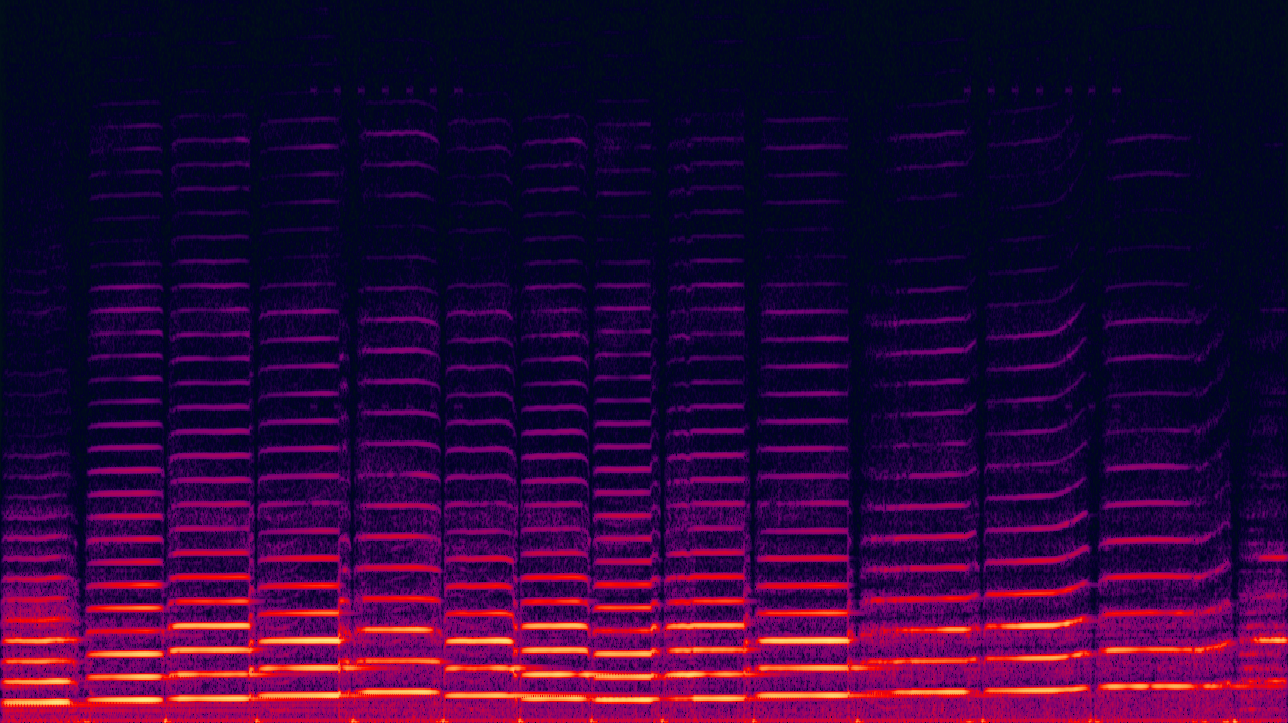
\includegraphics[width=0.8\linewidth]{Figures/Spectrogram.png}
	\caption[Spectogram of a file audio]{Spectogram of a file audio. Image owned by \url{https://en.wikipedia.org/wiki/User:Omegatron}, used under Creative Commons Attribution-Share Alike 3.0 Unported (CC BY-SA 3.0) licence \url{https://creativecommons.org/licenses/by-sa/3.0/deed.en}.}
\end{figure}

\noindent Another potential application of the clustering-based comparison method is the analysis of literary works, where the input is generated using word embeddings. These algorithms convert text into sequences of real vectors that capture semantic proximity. This approach improves the pre-processing, and by using a pre-trained transformer, it is possible to extract more complex semantic meanings from large portions of text. This variant allows the \gls{cada} method to be used effectively, unlike the \gls{dada} method, which is limited to discrete entities such as alphabetic characters.

\noindent As part of this thesis, it would also be interesting to evaluate the attribution performance on colour or greyscale images containing drawings rather than just handwriting. In addition, different colour spaces could be explored, such as comparing \gls{rgb} with \gls{hsl}, or using logarithmic greyscale mappings, which might better separate clusters and improve the accuracy of the analysis.

\noindent Another interesting idea for changing the nature of the input to image analysis is the use of Peano curves. This technique, while not entirely new, has been explored in the context of applying one-dimensional data mining operations to images.\footnote{For more about Peano curves and their application to image analysis, see \\ \url{https://deepai.org/publication/space-filling-curves-for-high-performance-data-mining}} Specifically, the image is transformed into a single continuous line of grey pixels representing the Peano curve. The algorithm can then be applied to this line as if it were a sequence of characters.

\subsection{CADA with GMM}
As previously mentioned, this thesis explores a generalisation of \gls{dada} through \gls{cada}, applied using \gls{kmeans} and \gls{fcm}. Additionally, the \gls{gmm} clustering algorithm was briefly introduced, which operates on a fundamentally different principle compared to \gls{fcm}. Investigating this type of clustering to compare two works could also be of interest. Specifically, \gls{gmm} clustering aims to approximate the unknown original density of the sample sets with a known one.

\noindent As explained in \cref{chap:LiteratureReview}, given a set of samples $A\subset\mathbb{R}^K$, the \gls{gmm} algorithm estimates the parameters $p_i\in \mathbb{R}$, $\Sigma_i\in\mathbb{R}^{K\times K}$, and $\mu_i\in\mathbb{R}^K$ for each cluster $i$. These parameters describe the following process for generating A:
\begin{enumerate}
	\item Select a cluster $i$ with probability $p_i$.
	\item Sample a point from the multivariate Gaussian distribution $\mathcal{N}\left(\mu_i,\Sigma_i\right)$.
\end{enumerate}

\noindent So the density approximating $A$ is given by
\[
f(x) = \sum_i p_i\phi_i(x)
\]
where $\phi_i(x)$ is the density of the $i$-th multivariate Gaussian at $x$:
\[
	\phi_i(x) = \left(2\pi\right)^{-k/2}\det\left(\Sigma_i\right)^{-1/2}\exp\left(-\frac12\left(x-\mu_i\right)^T\Sigma^{-1}\left(x-\mu_i\right)\right)
\]

\noindent In \cref{eq:SapAttribution_dist} we can define $f_{A}(x)$ as the density suggested by \gls{gmm} to approximate the set of samples $A$, and similarly $f_B(x)$ for $B$. Naturally, the comparison function between two set of samples can then be rewritten as
\[
	d(A,B)=(1+J_{D_A, D_B})^{-1} \times \int dx\left(\frac{f_A(x)-f_B(x)}{f_A(x)+f_B(x)}\right)^2
\]
\noindent Note that defining the Jaccard index in the context of \gls{cada} with \gls{gmm} is not simple. However, since explicit densities are being used, it may be useful to see if a highly accurate numerical estimate of this integral can be provided. This is undoubtedly a stimulating theoretical challenge.

\subsection{Understand the author}
An analysis not addressed in this thesis is the identification of the tiles that contribute most to the result of a comparison. Since the \gls{cada} method constructs clusters and assigns more weight to the least represented ones, it might be interesting to elaborate on the concept of the weight of a tile and highlight these tiles in the two compared images.

\noindent In particular, starting from \cref{eq:fuzzy_distance}, one could consider the clustering \gls{fcm} fixed and assign a weight to each centroid $c$. Subsequently, this weight could be transferred to the tiles according to their membership. The expectation is that the tiles that are most involved in the author's writing are those that contribute the most to the comparison.

\noindent Further analyses could include the study of centroids, such as identifying those typical of a specific author or those generally irrelevant. This type of analysis could lead to new ways of comparison based on centroids. For example, it could be discovered that centroids with values close to $(1,\ldots,1)$ are insignificant. Consequently, the synthesis could exclude clear tiles, slightly sacrificing attribution accuracy but considerably increasing computational performance.

\subsection{Attribution}
An important aspect to emphasise is that the results of this thesis were mainly evaluated in terms of attribution ability. However, only one attribution technique has been adopted in this paper, and it is rather elementary. An interesting analysis could consist in identifying which works of each author played a key role in the attribution. For instance, it might be useful to note which works provided the greatest number of true positives for their author. This analysis would not only improve the effectiveness of attribution, but also help speed it up, as well as provide useful information on the authors.

\noindent A further method to optimise the analysis concerns the study of the relationship between the comparison value between two works and a possible distance. Although, as stated in \cref{eq:SapAttribution_dist}, the comparison function is not a distance in the mathematical sense, there may be an upper bound for the comparison value between two works based on the other comparisons.

\noindent In practical terms, if $d(A,B)$ and $d(B,C)$ are very small, does it make sense to assume that $d(A,C)$ will also be small? For example, if one could establish a relation of the type $d(A,B)+d(B,C) \geq d(A,C)^\frac12$, one could obtain a useful criterion to reduce the calculations needed in attributions, significantly speeding up the process. This idea deserves further theoretical investigation to verify its validity and applicability.

\subsection{Neural Networks}
Another interesting type of analysis consists in comparing the method with neural networks, in particular with convolutional networks followed by a Multi-Layer Perceptron (MLP). These models examine images in a strikingly similar way: both analyse small tiles extracted from the image as initial input, and then apply aggregation or clustering to generate the final output. Although the explicit calculations differ significantly, the fundamental ideas behind the two approaches have similarities.

\noindent It would be interesting to explore possible connections between the two models and assess whether there is a synergy that could be exploited in practical applications. For instance, a neural network could be used to improve the synthesis or attribution phase, or to refine the clustering of \gls{cada} based on automatically learned features. This direction could open up new possibilities to combine the strengths of both approaches and develop more robust and efficient methods.

\section{Conclusions}
This thesis introduced a new approach to move from analysis methods on discrete distributions, such as \gls{dada}, to analysis on continuous distributions, such as \gls{cada}. Using clustering, it was possible to dynamically discretise a continuous space, overcoming the limitations of static methods and improving high-dimensional robustness. In particular, the use of \gls{fcm} allowed the clusters to be flexibly adapted to the data, improving the ability of the method to deal with noise in the data.

\noindent During the course of the work, I developed a complete system for image management and analysis, integrating preprocessing, image synthesis and clustering comparison steps. I implemented an efficient version of the clustering \gls{fcm} on \gls{gpu}. In addition, image cleanup techniques, such as the square grid, have been investigated using \gls{fft}.

\noindent The comparison function based on \gls{fcm} opens up new possibilities for the analysis of distributions of different natures. In addition to images, the method can be applied to written texts, through Word Embedding techniques, and to audio files, thanks to spectral representations. This significantly extends its application potential.

\bigskip \noindent This thesis represents a contribution to the field of graphics analysis, introducing a new method based on dynamic clustering, which has proven effective in realistic and challenging contexts. However, some limitations were highlighted, such as the dependence on preprocessing and high computational costs for large datasets. These aspects offer insights for further improvements, including optimisation of computational pipelines and reduction of preprocessing dependency.

\noindent Future prospects include the extension of the method to other types of data, such as colour images and audio samples, as well as the integration with machine learning techniques to further automate the analysis and improve the scalability of the system.

\bigskip \noindent In conclusion, this work has shown that complex problems in the attribution of graphic works can be successfully addressed through methodological innovation, offering insights for further research and applications in the field.
\end{toReview}
